%\input{preamble}
\documentclass{article}
\bibliographystyle{plainnat}
\usepackage[english]{babel}
\usepackage[latin1]{inputenc}
\usepackage[numbers]{natbib}
\usepackage[]{graphicx} %dvips
\usepackage[]{subfig}% Need to make several pictures in one float
\usepackage{verbatim} %% For Comment enviroment
\usepackage{lastpage}  % gives lastpage commando
\usepackage{algorithm}  %%% Algorithm Eviroment
\usepackage{algorithmic}  %%% Algorithm Eviroment
\usepackage{amsmath,amsfonts,amssymb,amsthm} % Math Paths
\usepackage{fancyhdr} % For headers
\usepackage{xifthen}% provides \isempty test and ifthen else 
\setcounter{tocdepth}{1}
\linespread{1}

\begin{document}

%Forside
\thispagestyle{empty}
\begin{center}        % Sentrerer teksten
  %Tittel
  \vspace{5mm}          % Vertikalt mellomrom
  \LARGE
  \textbf{Mini Project in Programming} \\
  \Large
  \vspace{5mm}
  \textbf{by} \\
  \vspace{5mm}
  %Forfatter
  \large
  \textbf{swI} \\
  %Avdeling for mekanikk
   \vspace{2mm}
  %%%%%%%OLD%%%%%%{\bf{\textsl{CANDIDATUS SCIENTIARUM}}} \\
  {\bf{\textsl{}}} \\
  \vspace{5mm}
  {\large \textsl {}}\\


		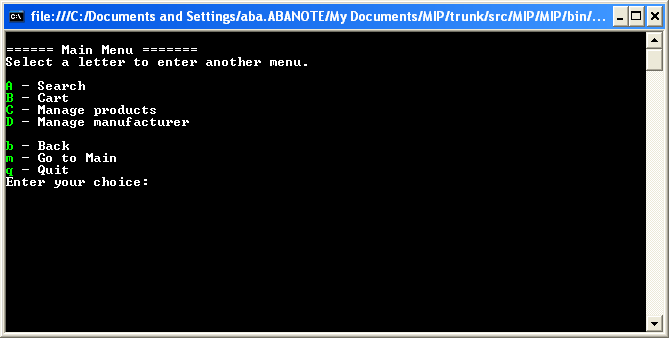
\includegraphics[width=\textwidth]{Main}

	  
  %Maaned, aar
  \vspace{10mm}
  \large
  \textsl{Fall 2010} \\
  \vspace{10mm}

	\large
  Kristian Kolding Foged-Ladefoged \\ \ \\
	------------------------------------------ \\ \ \\
	\large
  Kim Ahlstr�m Jakobsen \\ \ \\
	------------------------------------------ \\ \ \\
	\large
  Alex Bondo Andersen \\ \ \\
	------------------------------------------ \\ \ \\
\end{center}
\pagebreak

\section*{Our Program}
This brief piece of text describes what our program does(and vaguely how it does it) along with the decisions we have made for the requirements which were not clear to us in our assignment.

\subsection*{Before Running the Program}
Make sure to have the ``Init.txt'' file in the same directory as the executable ``MIP.exe'' in order to load products and manufactures.

\subsection*{Running the Program}
Our program manages manufacturers, products and a cart.
Each product must have a manufacturer.
It is possible to add and delete both products and manufactures in our program.

Each menu is build the same way.
Each line of a menu contains an ``identifier'', and a text string.
The identifier is a string which the user can enter to execute the method belonging to the text string.

Each menu gets a back-, quit-, and main-command.
Back leads to the previous menu.
Quit asks the user if he/she wishes to quit, and does what the user tells.
The main-command returns to the main menu described below.

\subsubsection*{Main Menu}
The main menu is the root of the program so to speak, it leads to search, cart, and management of products and manufactures.
It is not possible to go back from the main menu.

\subsubsection*{Search Menu}
The search menu consists of two parts; a list of products and commands.
The identifiers for the members of the list of products are numbers.
Selecting a number adds the given product to the cart.
The commands uses upper case letters and allows the user to filter the list, e.g. by applying a price range or search for a product code.

It was not part of the assignment to make an upper bound for storage capacity, we did however add such a filter, to make the filter by capacity resemble the filter by price.

Notice that each search operation filters the list, i.e. the list is not reset before each operation.

\subsubsection*{Cart Menu}
According to the assignment, we should make sure only one cart exist, therefore the Cart class use the singleton dessign pattern.
The cart menu prints the content of the cart according to the specifications of our assignment.
Further the user may checkout his/her items, clear the cart, or remove a specific number of items from the cart through this menu.

\subsubsection*{Manage Products Menu}
From the menu the user can either add a new product or remove existing products.
The products added/removed only apply for the given run of the program, the changes are not saved to the ``Init.txt'' file.

To add a product it must comply with the specifications of the assignment, e.g. the price cannot be negative.

A product can always be removed, even if it is part of the cart.
It will however not show up in the cart after deletion.

\subsubsection*{Manage Manufacturers Menu}
From this menu the user can either add a new manufacturer or remove an existing manufacturer.
The manufacturers added/removed only apply for the given run of the program, the changes are not saved to the ``Init.txt'' file.

To add a manufacturer it must comply with the specifications of the assignment, e.g. the URL must start with ``http://''.

It is not possible to remove a manufacturer which is associated to one or more products, since this would result in a product without a manufacturer.

\subsection*{Error Handling}
We have used many try-catches throughout our program.
Our catch statements takes only specific exceptions in order to avoid catching an exception which should not have been caugth.
In our Initialize method there is a try-catch around MainMenu, which catches every exception and prints the stack trace and then runs the MainMenu again, to avoid the program crashing for the user.
It could perhaps been made in a way such that the user is alarmed with the error where it occurs instead of returning to the MainMenu.

\subsection*{Sources}
We used http://msdn.microsoft.com/en-us/library/ to lookup classes and functions we were unsure about.

\end{document}